%!TEX root = Main.tex
\documentclass[Main]{subfiles}

\begin{document}
\section{Convolutional Neural Network Method} % (fold)
	\label{sec:convolutional_neural_network_method}
	In this section I describe how I tried to implement a system for detecting pain in faces using a Convolutional Neural Network.
	I did not succeed in creating a working proof-of-concept in the time I had available for this project, but I will describe what I tried and what I learned below.
	% \fxnote{Revisit this part when done with the rest} 

	\subsection{CNN Basics} % (fold)
		\label{sub:cnn_basics}
		Convolutional Neural Networks are a class of deep Artificial Neural Networks (ANN).
		A traditional feed-forward ANN consists of layers neurons and biases.
		These are fully connected by a set of weights that are trained by backpropagation (See Figure \ref{fig:ufldl_ann}).
		\begin{figure}[H]
			\begin{center}
				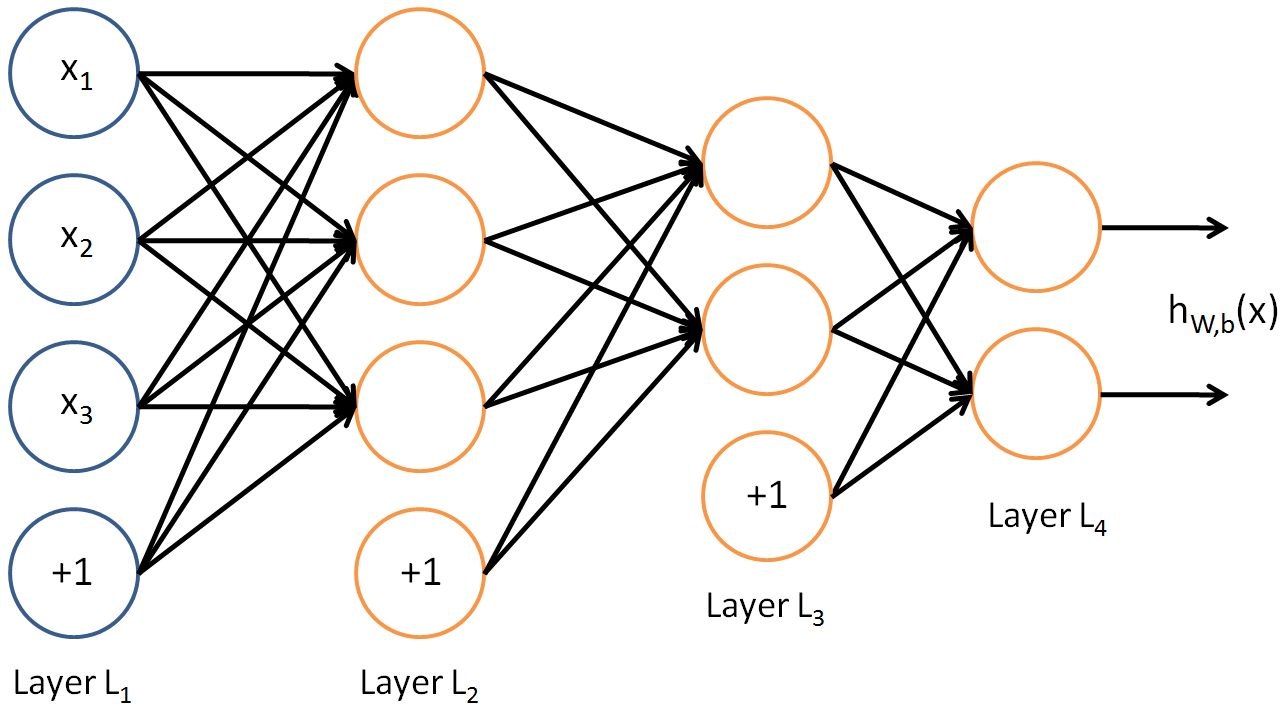
\includegraphics[width=0.45\linewidth]{UFLDL_ANN}
			\end{center}
			\caption{Illustration of a simple ANN, taken from \cite{ufldl}.}
			\label{fig:ufldl_ann}
		\end{figure}

		In CNNs the weights are instead sets of filter kernels that are convolved with the input image, hence the name.
		This reduces the amount of parameters to train because the weights are shared for all the pixels in an input.

		Between the filter neurons there are typically pooling layers inserted.
		These serve to further reduce and concentrate the data in the network.
		They work by nonlinearly sub-sampling the output image of a filter layer by eg. only sampling the pixel of highest intensity in each $2\times2$ pixel patch of the image (See Figure \ref{fig:lisa_cnn}).
		This also makes them more tolerant to small translations of the input image.
		\begin{figure}[H]
			\begin{center}
				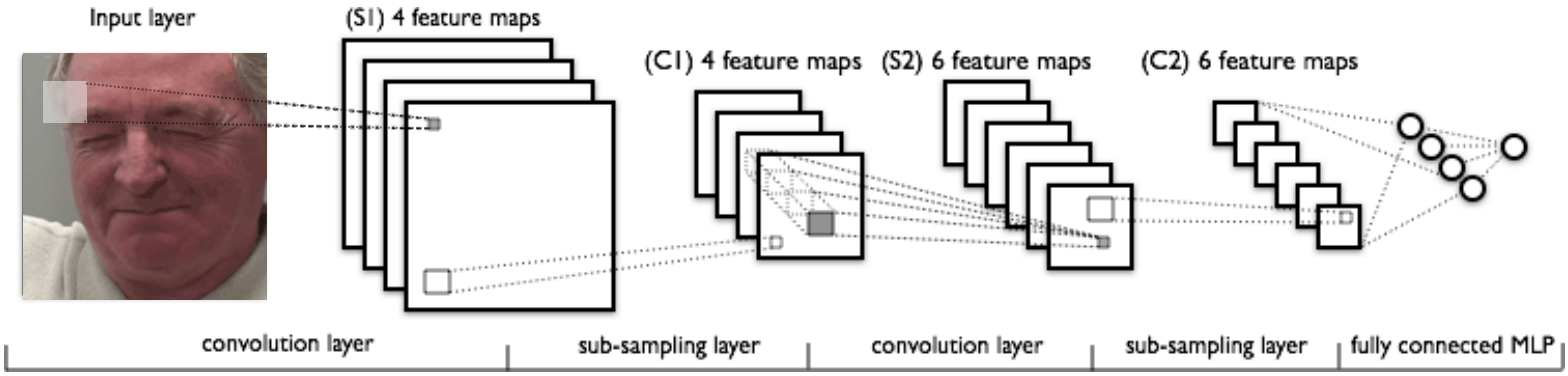
\includegraphics[width=0.8\linewidth]{CNN_example}
			\end{center}
			\caption{Illustration of a simple CNN, taken from \cite{LISAlab2015}.}
			\label{fig:lisa_cnn}
		\end{figure}
		
		The final classification is then done by either an SVM or one or more layers of traditional fully connected ANN layers like shown in Figure \ref{fig:lisa_cnn}.


		% subsection cnn_basics (end)
	
	\subsection{CNN Libraries/Toolboxes} % (fold)
		\label{sub:cnn_libraries_toolboxes}
		I have tried a couple of different libraries and toolboxes to implement the CNN:
		
		\subsubsection{DeepLearnToolbox} % (fold)
			\label{ssub:deeplearntoolbox}
			DeepLearnToolbox \cite{IMM2012-06284} is a toolbox for MATLAB, completely written in MATLAB by Rasmus Berg Palm, as part of his masters thesis at DTU.
			This toolbox offers a wide variety of functions within the domain of Deep Learning.

			This toolbox was my first attempt at implementing a CNN for pain recognition.
			I was able to install the toolbox and run test and example scripts without issue, but I never got any good results for my application.
			The problem was that with my data, processing was very slow.
			It took several hours to train a single epoch, making it next to impossible to make any progress in my development.
			I attest these problems to the fact that everything ran in MATLAB, which is known to be inefficient at times, and also partly to my inexperience with designing and training CNNs.

			% subsubsection deeplearntoolbox (end)

		\subsubsection{Deep Learning for Saliency} % (fold)
			\label{ssub:deep_learning_for_saliency}
			As described in Section \ref{sub:related_works}, a system for predicting eye fixations using CNNs has been implemented.
			I tried briefly to use thier code \cite{Shen2012a}, but found quickly that it written very much was written with their application in mind, and did not easily generalize. 

			% subsubsection deep_learning_for_saliency (end)

		\subsubsection{MatConvNet} % (fold)
			\label{ssub:matconvnet}
			MatConvNet \cite{Lenc2014} is an Open-Source MATLAB toolbox for CNNs written by \emph{vlfeat.org}, known for their excellent Computer Vision toolbox for MATLAB.
			The toolbox is implemented efficiently in C++ and in CUDA for GPU acceleration on NVIDIA hardware.\footnote{
				See Appendix \ref{sec:gpu_acceleration_of_cnn_training} for more on how to enable GPU acceleration with MatConvNet
				} 
			The code is compiled locally and have \texttt{.mex} wrappers so that it can be executed from MATLAB like any other MATLAB function.
			This is the toolbox I the majority of my time using.
		
			% subsubsection matconvnet (end)
		
		\subsubsection{Caffe} % (fold)
			\label{ssub:caffe}
			Caffe \cite{jia2014caffe} is much like MatConvNet a framework for implementing CNNs implemented in C++ and CUDA with tie-ins to MATLAB.
			Caffe seems to be the best freely available CNN framework at the moment, but an official port for Windows is not available yet, so using it was not an option for this project.

			% subsubsection caffe (end)

		% subsection cnn_libraries_toolboxes (end)

	\subsection{Method} % (fold)
		\label{sub:cnn_method}
		% Selection of toolbox
		% Work from example
		% Different tests
		The overall idea for my system is described in Section \ref{sub:proposed_approach}.
		After initial tests with different toolboxes I chose to work with the MatConvNet toolbox from VLfeat for the CNN part of the implementation.
		
		\subsubsection{Viola-Jones Face Detector} % (fold)
			\label{ssub:viola_jones_face_detector}
			A Viola-Jones face detector was implemented in MATLAB using a \emph{CascadeObjectDetector}.\footnote{See Appendix \ref{sec:code} - \texttt{ViolaJonesPatchExtract.m} for full MATLAB implementation.}
			This was used to locate the face of the subjects in all the frames.
			For a few of the frames the detector would have detections aside from the actual face eg. small patches around the neck or in the background.
			Also, sometimes it would not detect a face if subject was wearing glasses.
			To help with this, a minimum size for detection was set to $100\times100$ pixels.
			This is easily enough to detect a the actual face, but reject most of the other erroneous detections.
			After this only a very small amount of frames had erroneous detection.
			Therefore is was elected to just drop the frames that did not have exactly one detection, in stead of manually going through all the data.

			The location of the face is marked by a simple bounding box of coordinates.
			The patch within this box is extracted, converted to gray scale and resized to a common size.
			Both sizes $48\times48$ pixels and $100\times100$ pixels were tried.

			The position, rotation and scale of the face inside this patch could vary.
			Also the background is not extracted.
			This is because the plan is to train a robust CNN that adjusts for this itself, making the need for pre-processing in a final application minimal.

			% subsubsection viola_jones_face_detector (end)

		\subsubsection{MatConvNet Data Format} % (fold)
			\label{ssub:matconvnet_data_format}
			In order to use the MatConvNet toolbox the data has to be formatted in a certain way.\footnote{See Appendix \ref{sec:code} - \texttt{leaveOneOutData.m} for full MATLAB implementation.}
			Specifically the data has to be arranged in a layered \texttt{struct} called \texttt{imdb} (see Figure \ref{fig:imdb_struct}).
			This contains all the image data, the target labels, information on which samples are to be used for training/test/validation, along with some metadata.
			\begin{figure}[th]
				\begin{center}
					\includegraphics[]{imdb_structure}
				\end{center}
				\caption{Diagram of image database structure and contents}
				\label{fig:imdb_struct}
			\end{figure}
			
			The images has to be arranged in a 4D-matrix.
			The first two dimensions are the dimensions of the images (Rows/Columns).
			The next is a singleton dimension.
			This dimension is used when the input fans out into several feature maps.
			The last is the numbers of frames (N).
			\begin{equation}
				\texttt{imdb.images.data} \in \mathbb{R}^{R\times C\times1\times N} 
			\end{equation}
			All image data values are stored as \emph{single}-precision (32-bit) variables.
			This is typical for CNN data as it greatly increases computational speeds, especially with GPU acceleration.
			The mean image over all frames is also given as input data.

			\texttt{imdb.images.labels} is a vector of values, either 1 or 2 corresponding to the classes in \texttt{imdb.meta.classes} indicating if a frame is a positive or negative example.
			Likewise \texttt{imdb.images.set} is a vector of values, either 1, 2  or 3 corresponding to the classes in \texttt{imdb.meta.set} indicating if a frame is to be used for training, for validation or for test.

			In my case I only use a training and a validation set, and no separate test set.
			This does not cause any problems.
			The feature is just there so you can do cross validation on different sets of validation data and still save a separate test set.

			% subsubsection matconvnet_data_format (end)

		\subsubsection{CNN setup} % (fold)
			\label{ssub:cnn_setup}
			Being a novice in working with deep learning and CNN I chose to base my implementation on a working example that comes with the toolbox and adapt it to my application.

			The example base for my implementation was a network designed by the people behind MatConvNet to be similar to Yann LeCun's \emph{LeNet}.
			This example was made to classify hand written digits from the well know MNIST database \cite{mnistlecun}.

			The architecture of the net is defined by creating a \emph{struct} called \texttt{net} with fields corresponding to layers
			(See Listing \ref{lst:cnn_setup} or Appendix \ref{sec:code} - \texttt{cnn\_mnist3.m} for full script).
			Each layer is itself a \texttt{struct}, that defines its type, dimensions and initialization.

			\newpage
			\begin{lstlisting}[caption=Example of CNN setup, style=Code-Matlab, label=lst:cnn_setup]
	f=1/100 ;
	net.layers = {} ;
	net.layers{end+1} = struct('type', 'conv', ...
	                       'filters', f*randn(12,12,1,10, 'single'), ...
	                       'biases', zeros(1, 10, 'single'), ...
	                       'stride', 1, ...
	                       'pad', 0) ;
	net.layers{end+1} = struct('type', 'pool', ...
	                       'method', 'max', ...
	                       'pool', [2 2], ...
	                       'stride', 2, ...
	                       'pad', 0) ;
	net.layers{end+1} = struct('type', 'conv', ...
	                       'filters', f*randn(8,8,10,25, 'single'),...
	                       'biases', zeros(1,25,'single'), ...
	                       'stride', 1, ...
	                       'pad', 0) ;
	net.layers{end+1} = struct('type', 'pool', ...
	                       'method', 'max', ...
	                       'pool', [2 2], ...
	                       'stride', 2, ...
	                       'pad', 0) ;
	net.layers{end+1} = struct('type', 'conv', ...
	                       'filters', f*randn(4,4,25,250, 'single'),...
	                       'biases', zeros(1,250,'single'), ...
	                       'stride', 1, ...
	                       'pad', 0) ;
	net.layers{end+1} = struct('type', 'relu') ;
	net.layers{end+1} = struct('type', 'conv', ...
	                       'filters', f*randn(1,1,250,2, 'single'),...
	                       'biases', zeros(1,2,'single'), ...
	                       'stride', 1, ...
	                       'pad', 0) ;
	net.layers{end+1} = struct('type', 'softmaxloss') ;

			\end{lstlisting}

			Listing \ref{lst:cnn_setup} show the net I ended up using, after much tweaking and playing around with parameters.
			The net starts with a convolutional layer with one input (the image data), 10 output feature maps and a kernel size of $12\times12$ pixels.
			Next there is a max-pooling layer with a factor of $2\times2$.
			Next there is another convolutional layer with 10 input feature maps, 25 output feature maps and a kernel size of $8\times8$ pixels.
			Next, another max-pooling layer like the one before.
			Next there is another convolutional layer with 25 input feature maps, 250 output feature maps and a kernel size of $4\times4$ pixels.
			Next there is a layer Rectified Linear Units, followed by a fully connected convolutional layer.
			Finally, the last layer is a softmax loss layer.
			All the convolutional layers are initialized randomly and the biases are set to zero.

			There is also a set of hyper parameters to set before training can begin.
			These are defined in \texttt{struct} called \texttt{opts.train} as shown in Listing \ref{lst:cnn_hyper}.

			\newpage
			\begin{lstlisting}[caption=CNN setup hyper parameters, style=Code-Matlab, label=lst:cnn_hyper]
	opts.train.batchSize = 100 ;
	opts.train.numEpochs = 1000 ;
	opts.train.useGpu = false ;
	% opts.train.useGpu = true ;
	opts.train.learningRate = 0.0001 ;
	opts.train.momentum = 0.0;
	opts.train.weightDecay = 0.005 ;
			\end{lstlisting}

			% subsubsection cnn_setup (end)
		
		\subsubsection{Experiments} % (fold)
			\label{ssub:experiments}
				 
			% subsubsection experiments (end)		 



		% subsection cnn_method (end)
	

	


	\subsection{Results} % (fold)
		\label{sub:cnn_results}



		
		% subsection cnn_results (end)


	\subsection{Discussion} % (fold)
		\label{sub:cnn_discussion}
		

		% subsection discussion (end)

	% Noget om at det ikke kom til at virke
		% Hvad intensionen var
		% Hvilke værktøjer er anvendt
			% Sammenligning af værktøjer
		% Hvilke metoder er prøvet
		% Hvordan er netvæket sat op
		% Hvordan CNN overordnet virker
		% Mulige årsager til at det mislykkedes
			% For lidt data
			% For lidt tid
			% For lidt erfaring
			% Noget med autoencoder
			% Noget med opsætning af regularisereings parametere
			% Noget med hyperparametre
	
	% section convolutional_neural_network_method (end)

\end{document}